\chapter{Experimental}
\label{experimental}
\section{Model in the Loop}
\begin{figure}[h!]
    \begin{center}
    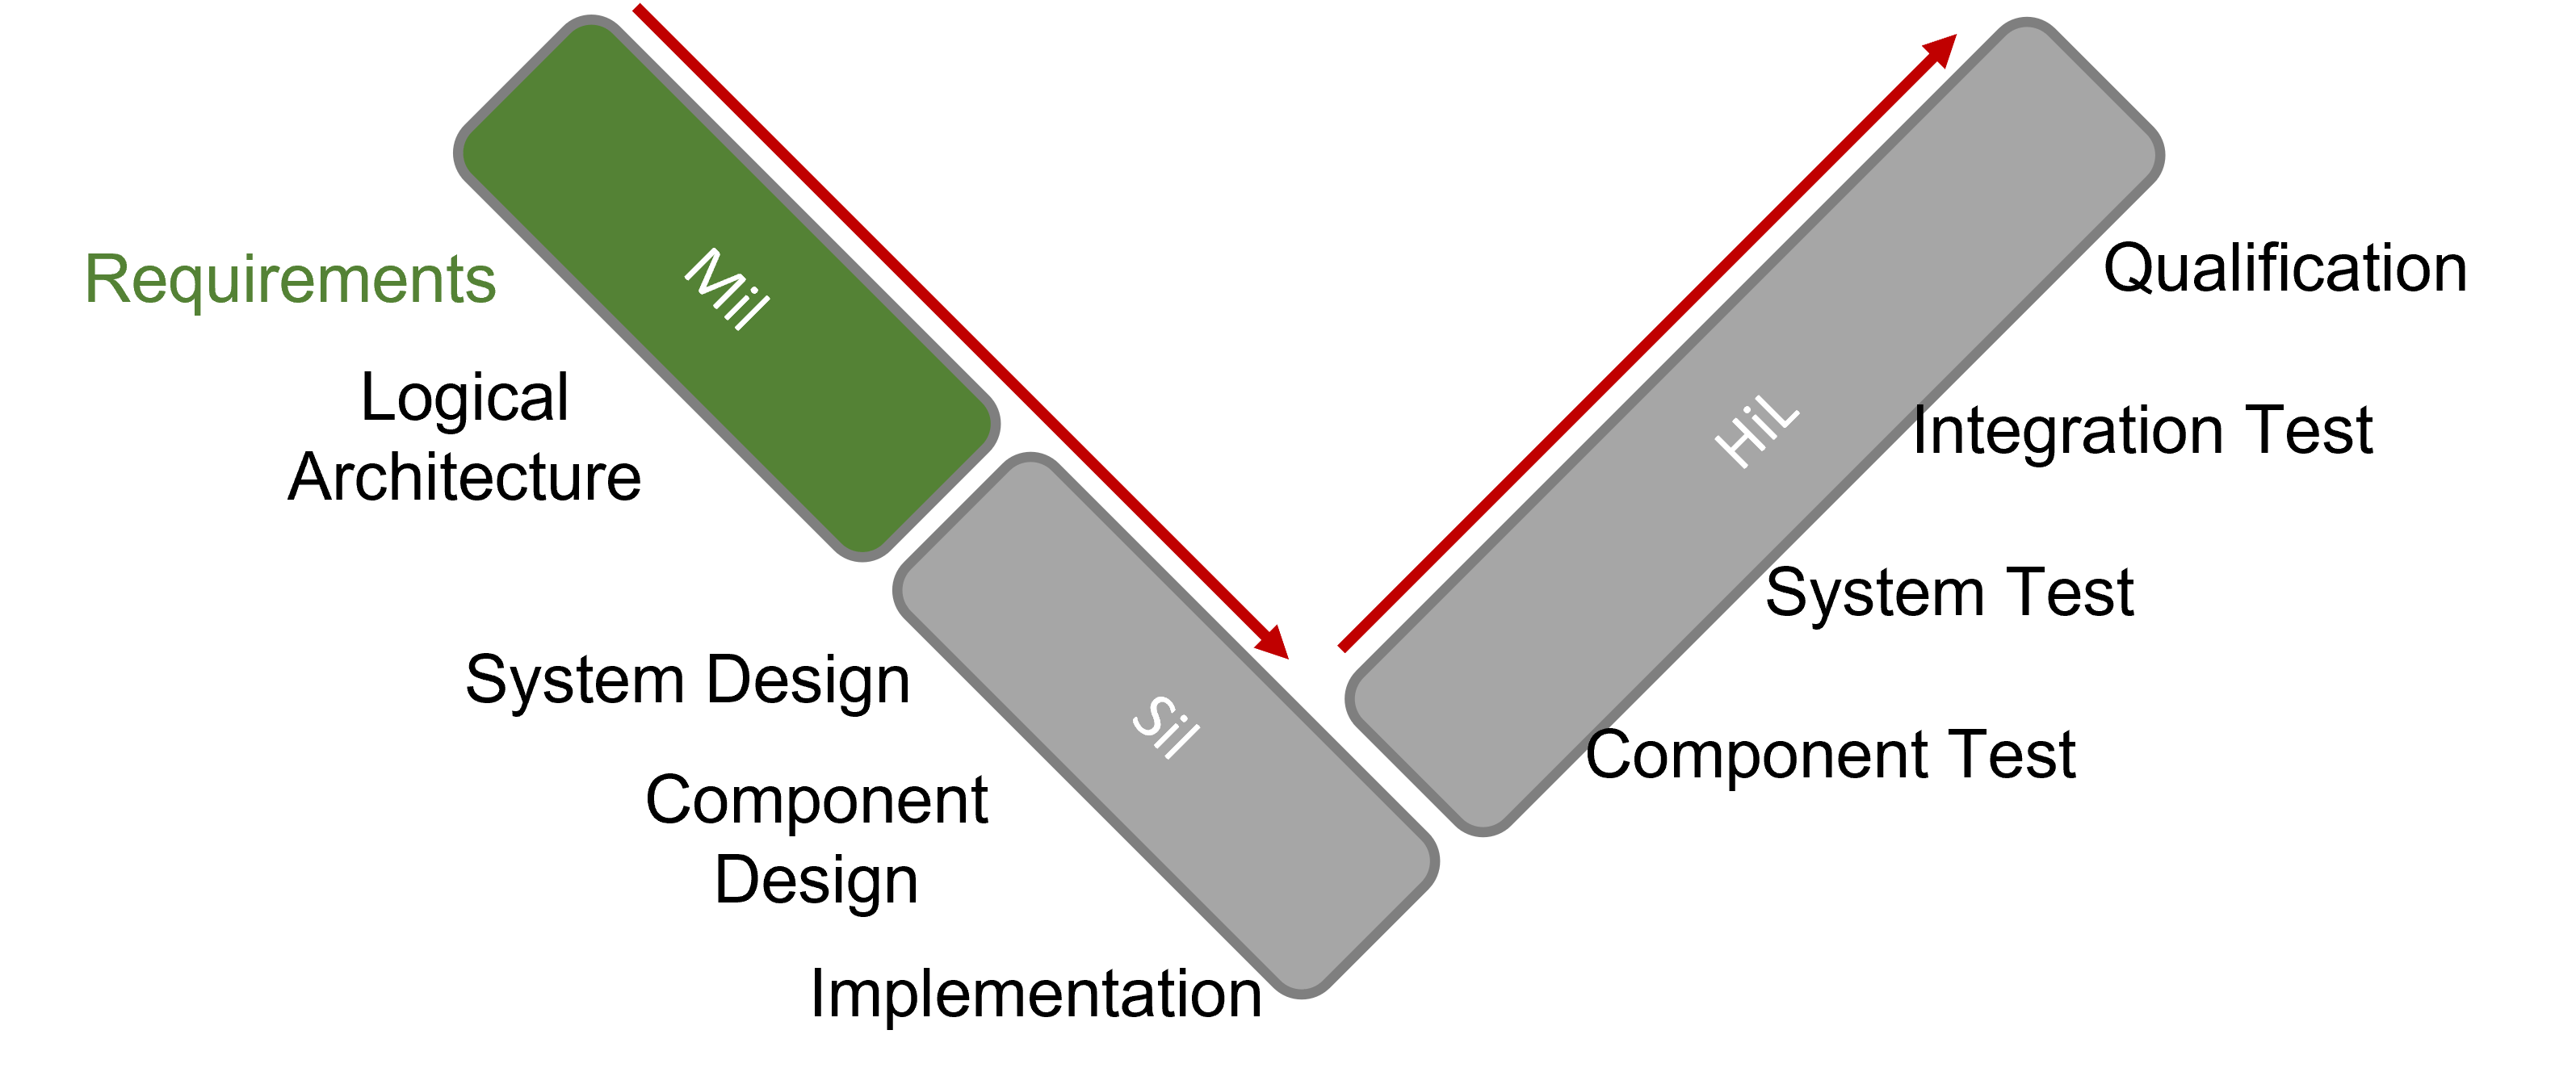
\includegraphics[width=12cm]{Pictures/V Model Requirements.png}
    \caption[V Model Requirements]{V Model Requirements Stage}
    \label{V Model Requirements}
    \end{center}
\end{figure}

\begin{figure}[h!]
    \begin{center}
    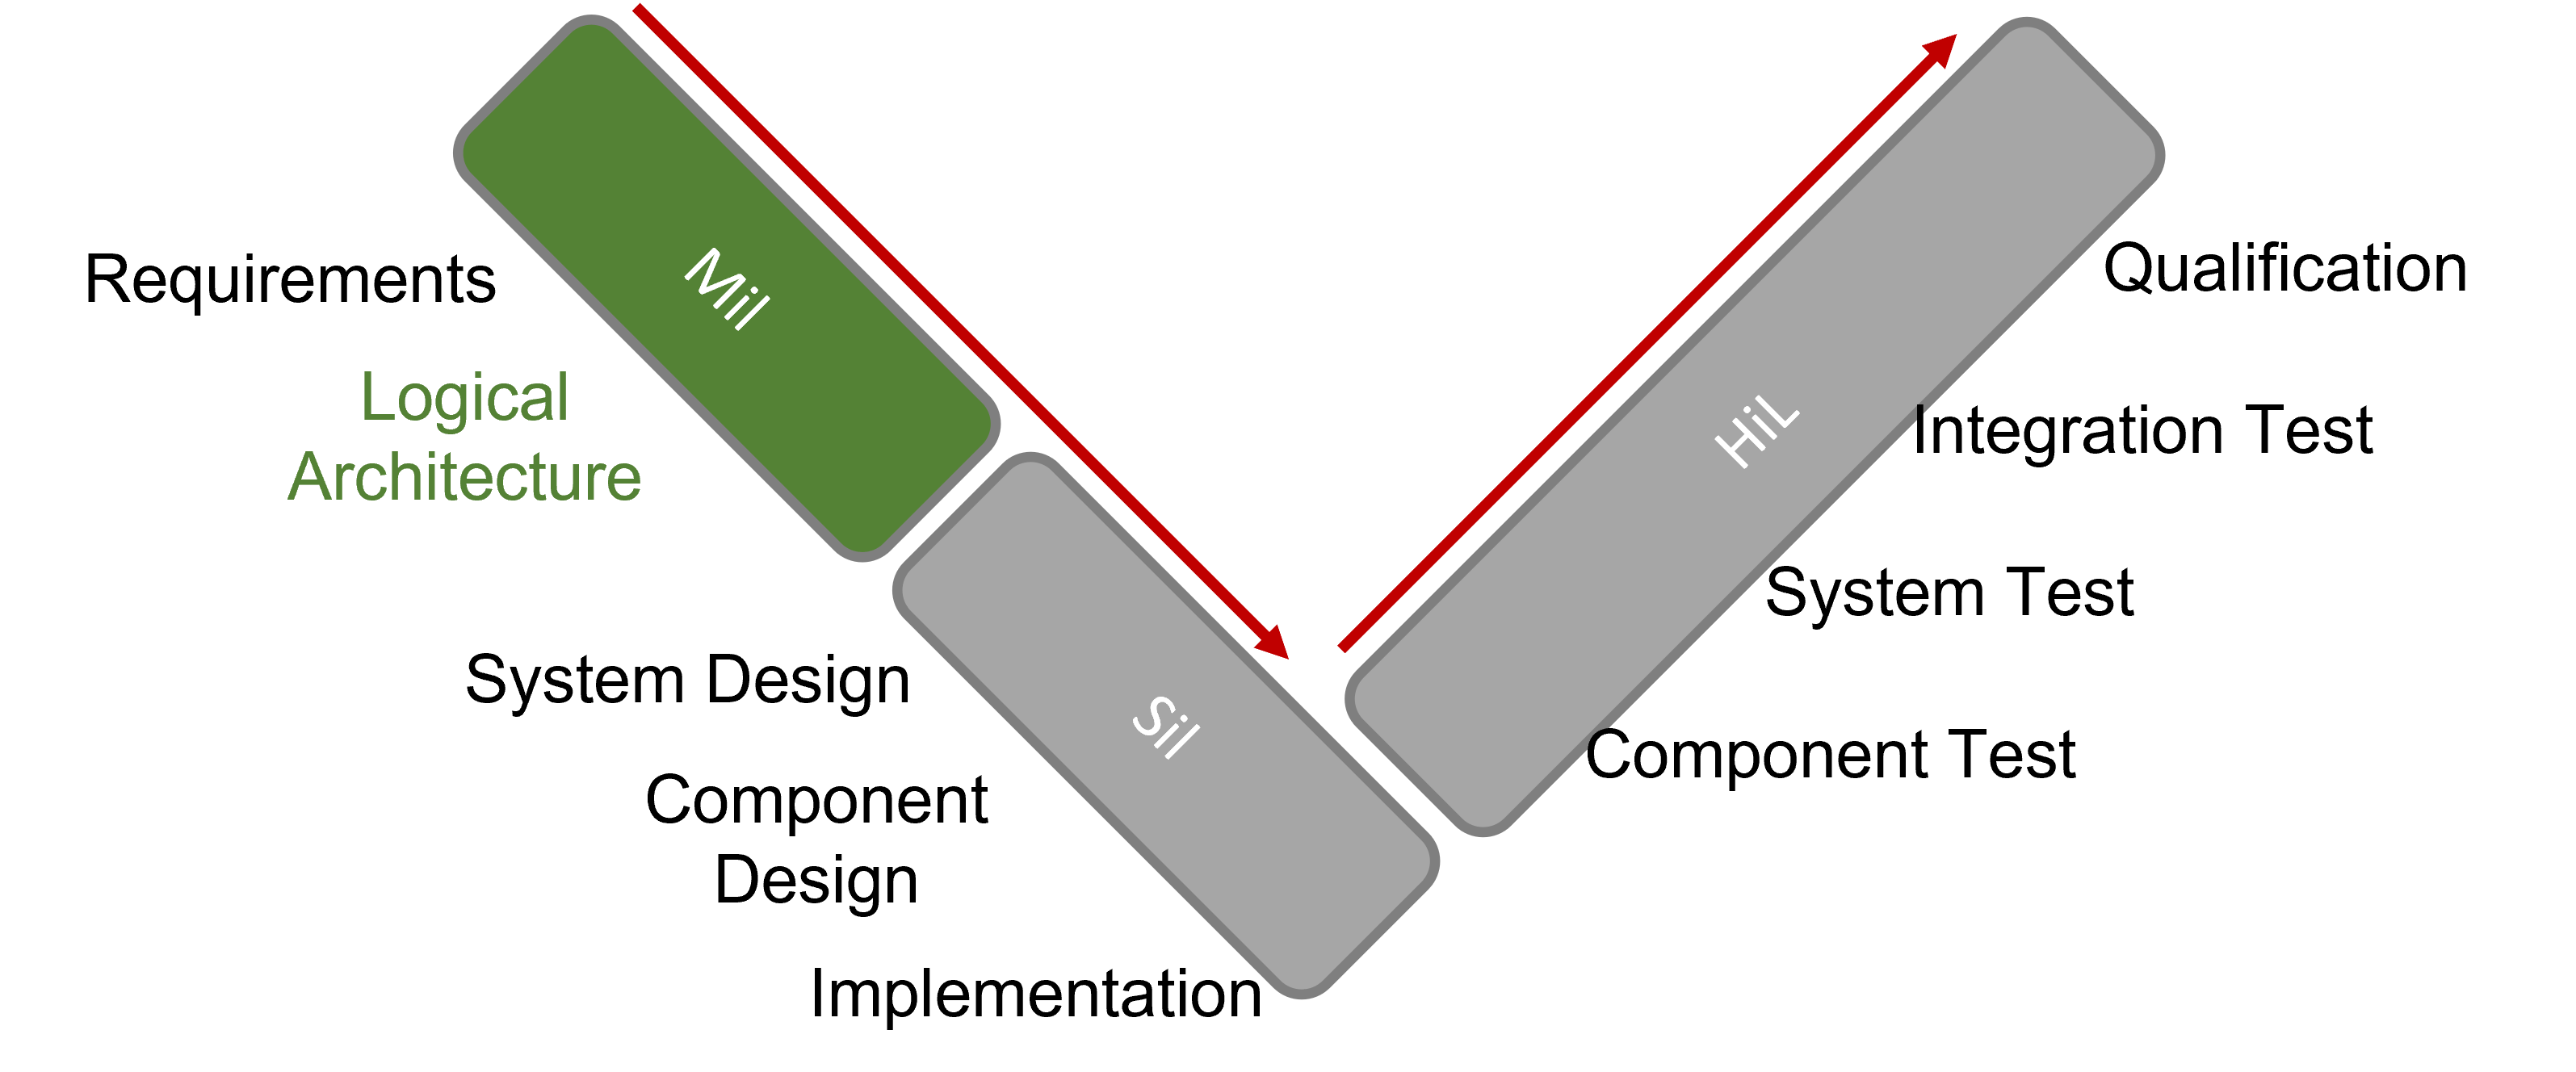
\includegraphics[width=12cm]{Pictures/V Model Logical Architecture.png}
    \caption[V Model Logical Architecture]{V Model Logical Architecture Stage}
    \label{V Model Logical Architecture}
    \end{center}
\end{figure}

\subsection{Initial Considerations}
\subsection{Parameter Identification}
\subsection{Simulink Model}
\subsubsection{Encoder and Spindel}
\subsubsection{Microcontroler}
\subsubsection{Stepper Motor}
\subsubsection{Gearbox}
\subsection{Code Generation}
\subsection{Mechanical Implementation}

\section{Software in the Loop}
\begin{figure}[h!]
    \begin{center}
    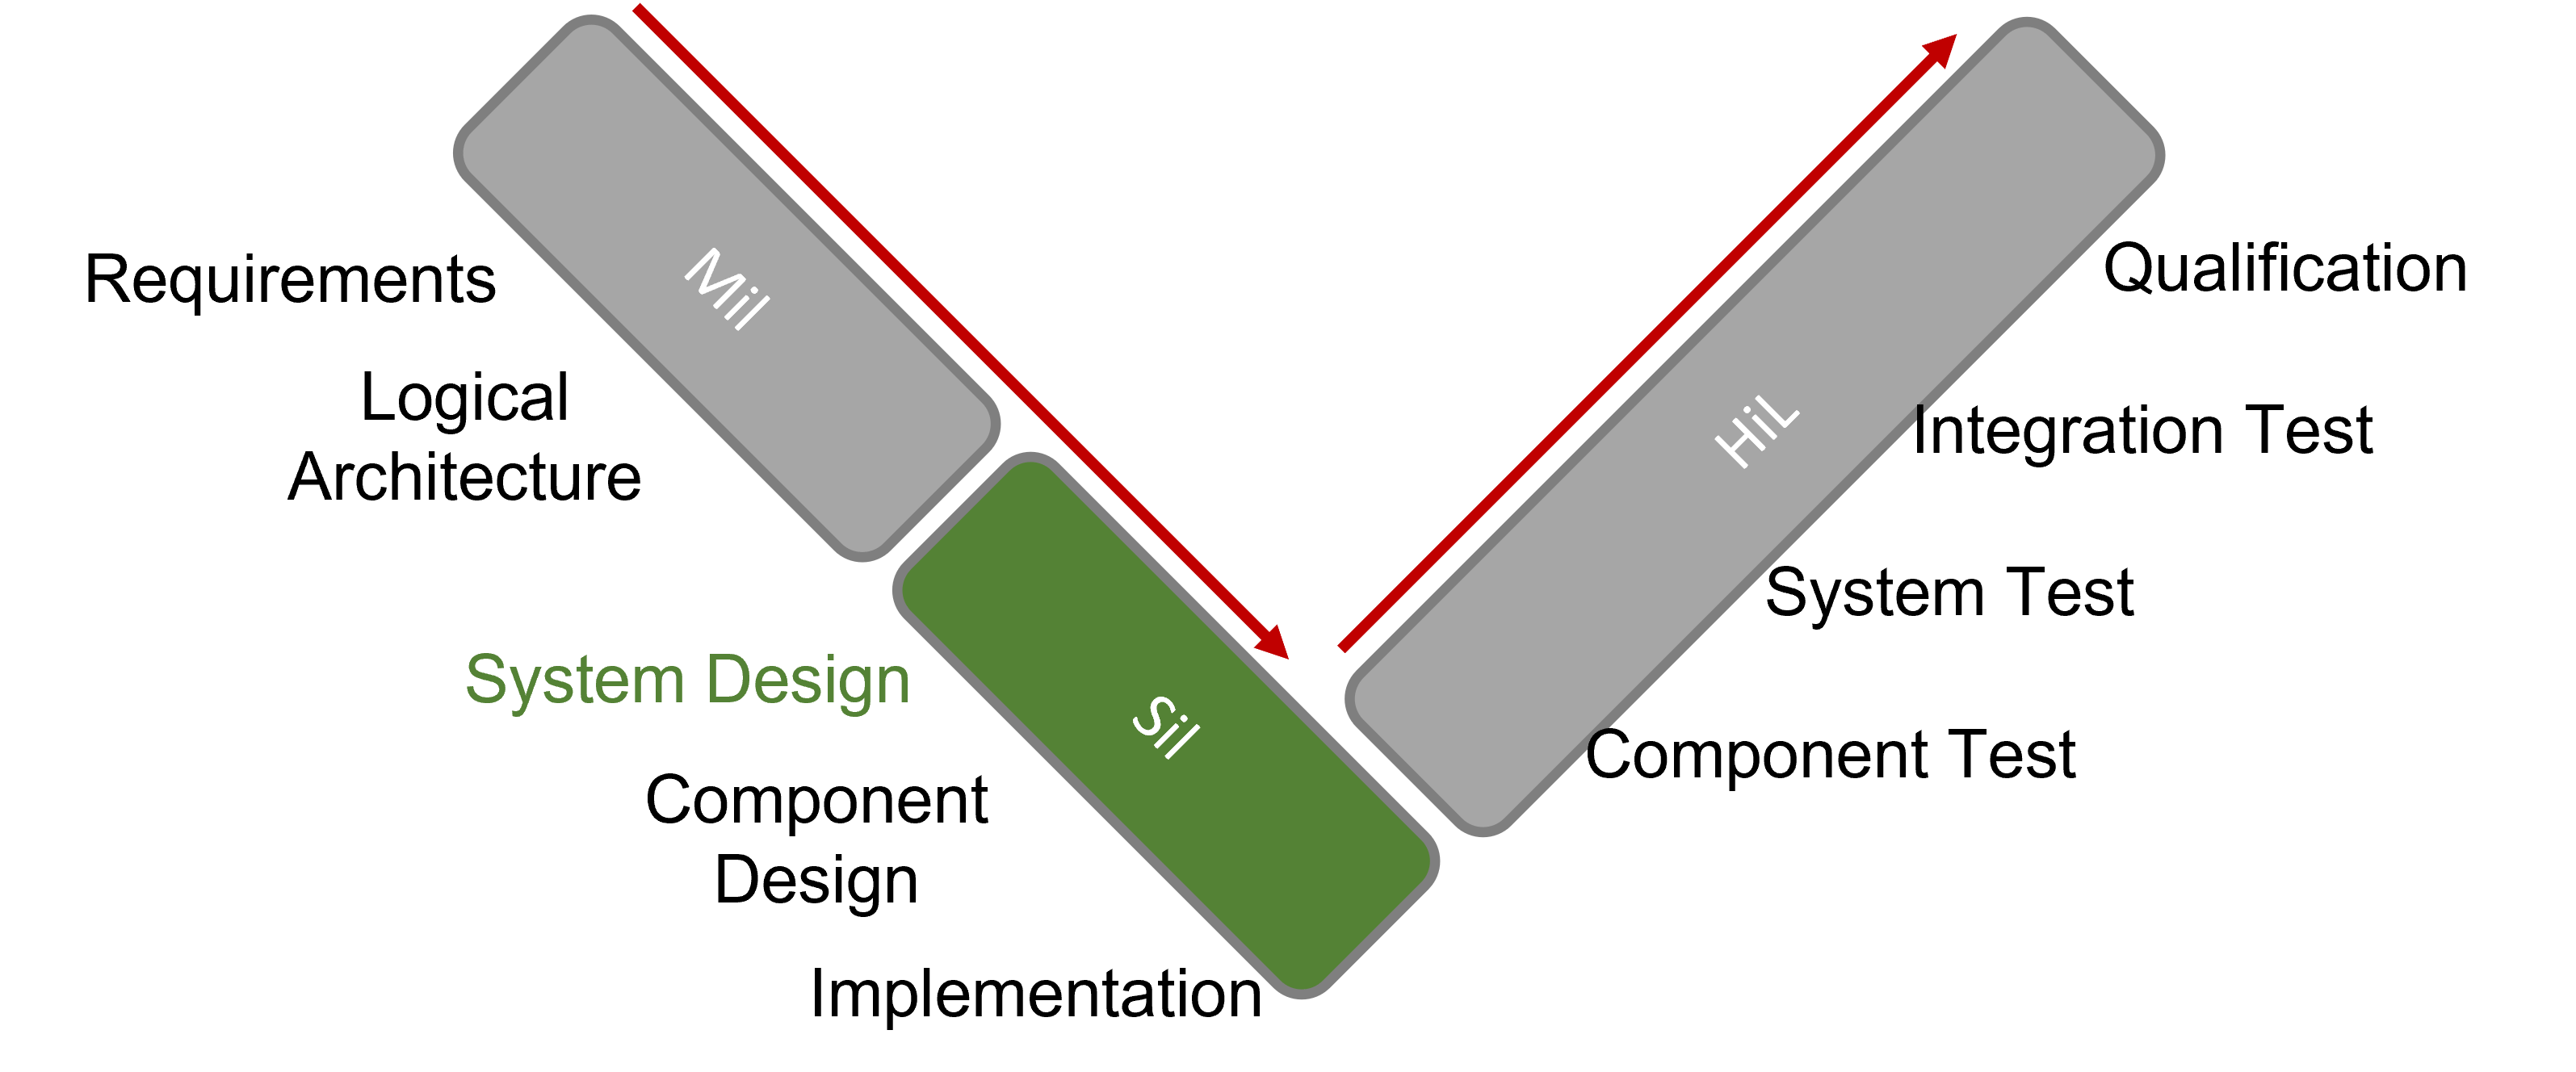
\includegraphics[width=12cm]{Pictures/V Model System Design.png}
    \caption[V Model System Design]{V Model System Design Stage}
    \label{V Model System Design}
    \end{center}
\end{figure}

\begin{figure}[h!]
    \begin{center}
    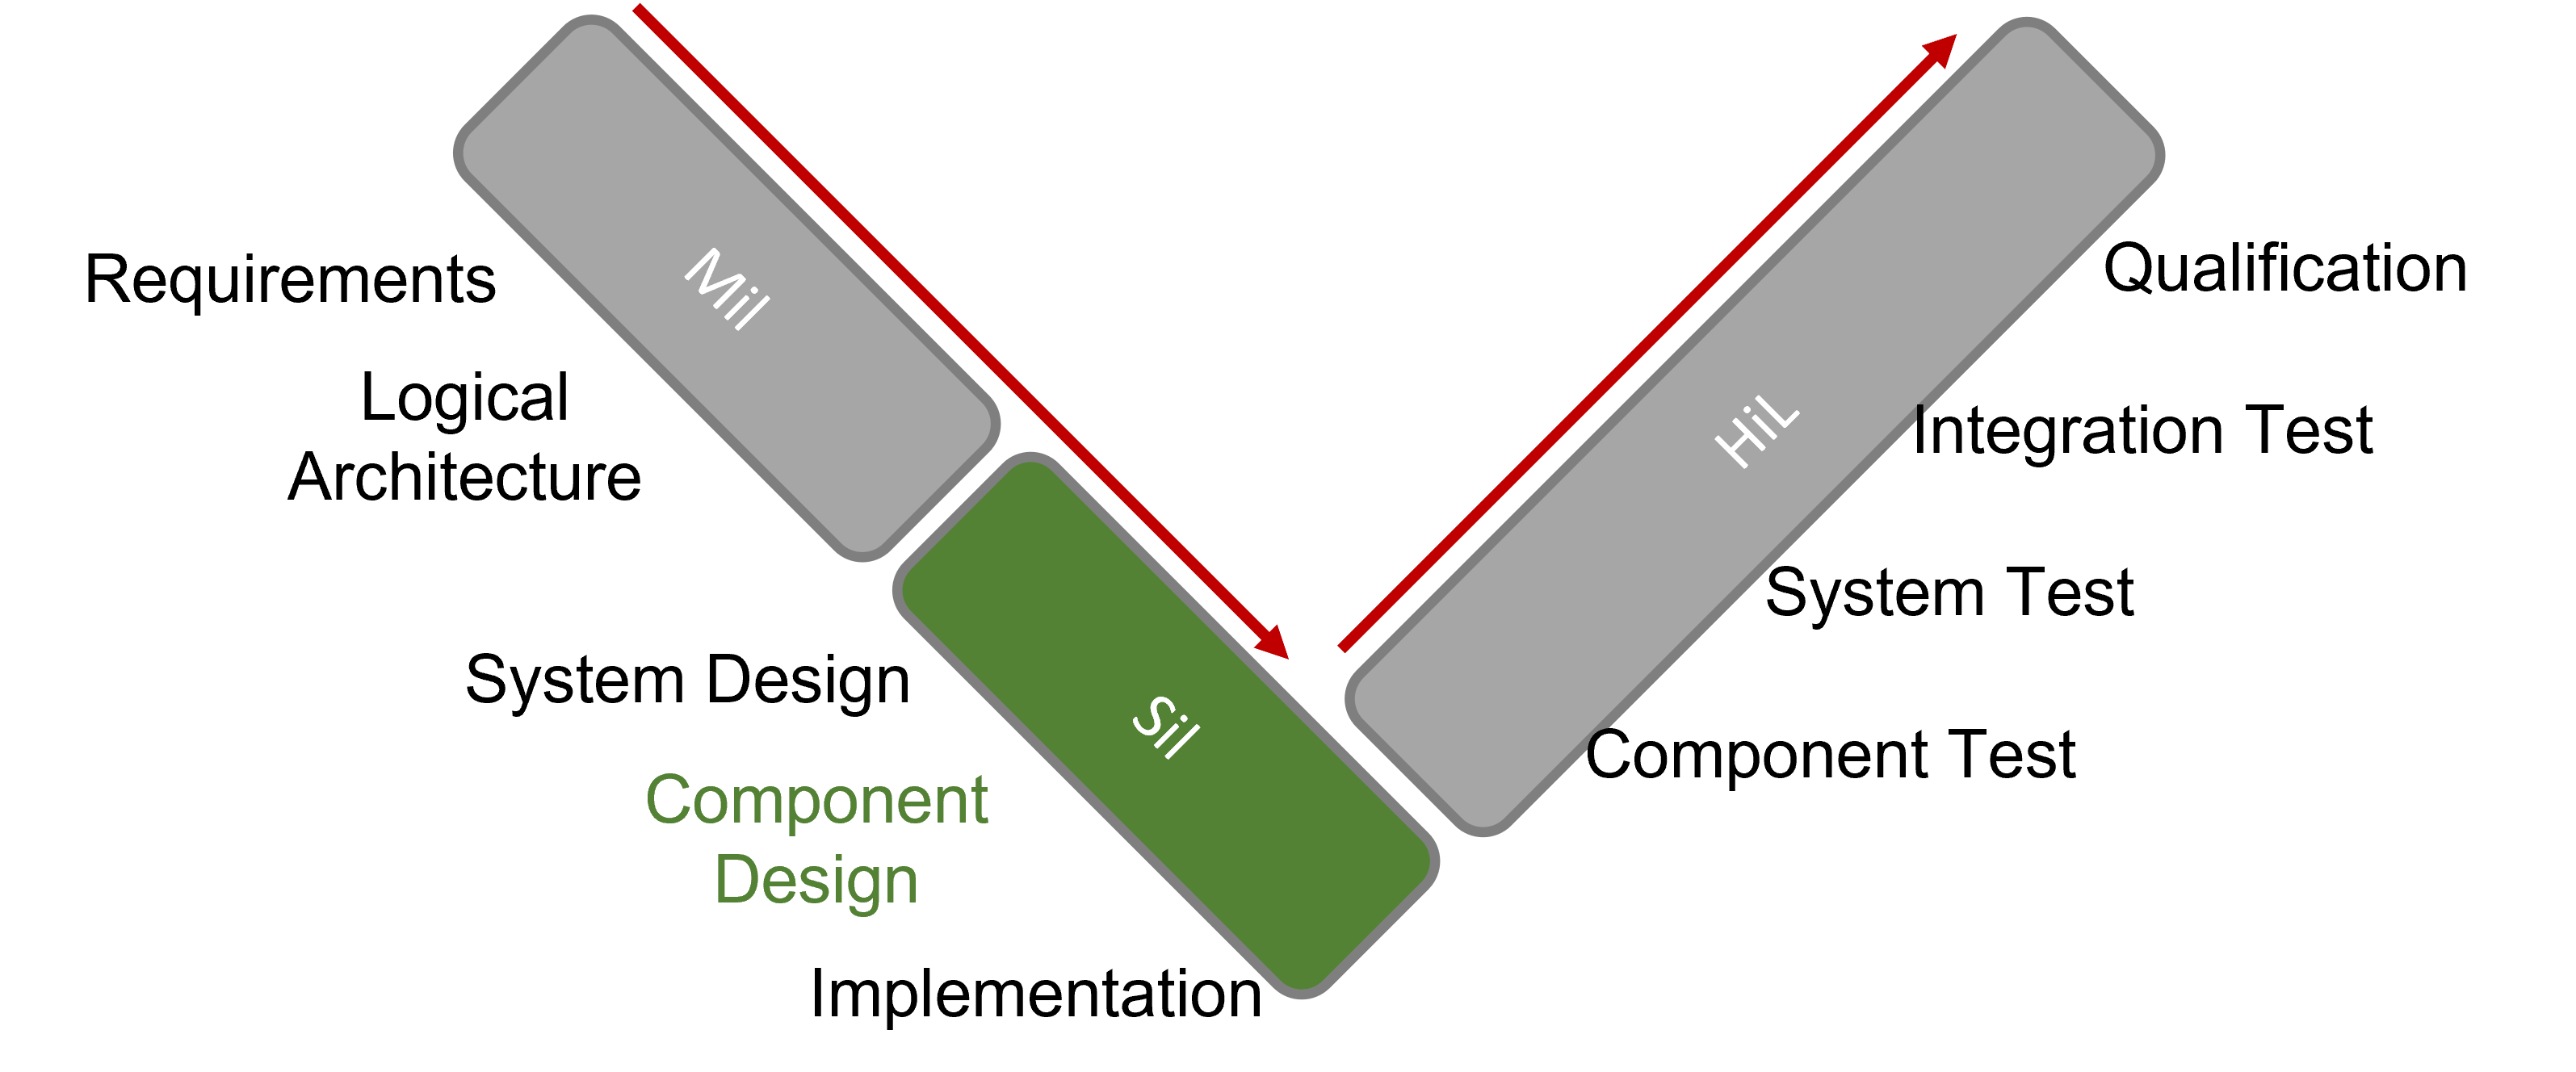
\includegraphics[width=12cm]{Pictures/V Model Component Design.png}
    \caption[V Model Component Design]{V Model Component Design Stage}
    \label{V Model Component Design}
    \end{center}
\end{figure}

\begin{figure}[h!]
    \begin{center}
    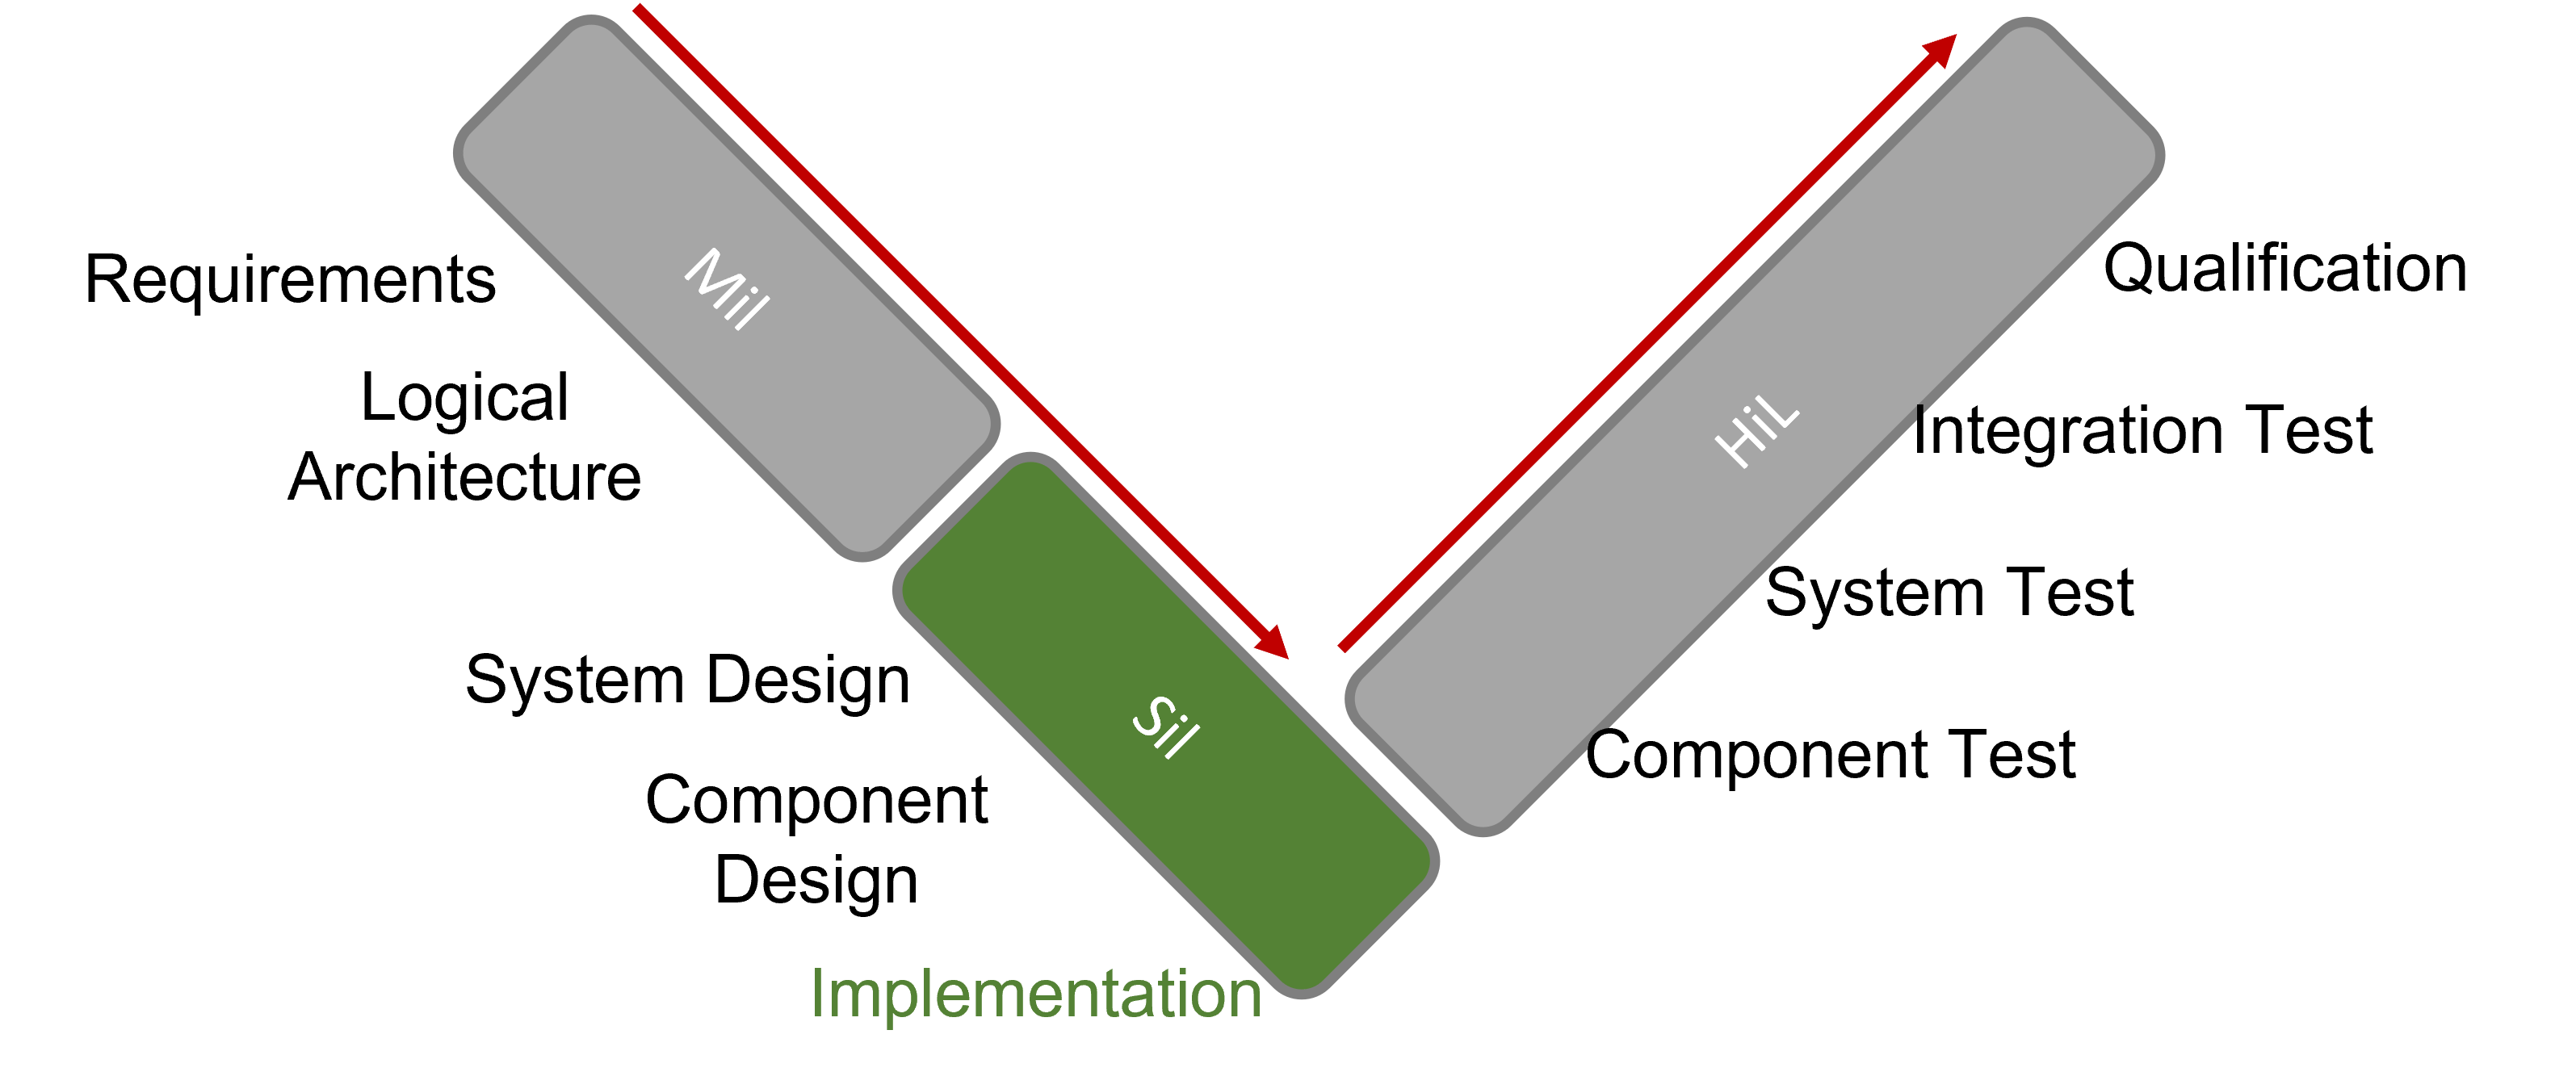
\includegraphics[width=12cm]{Pictures/V Model Implementation.png}
    \caption[V Model Implementation]{V Model Implementation Stage}
    \label{V Model Implementation}
    \end{center}
\end{figure}

\subsection{Logic}
\subsection{Arithmetic}

\section{Hardware in the Loop}
\subsection{Component Test}
\begin{figure}[h!]
    \begin{center}
    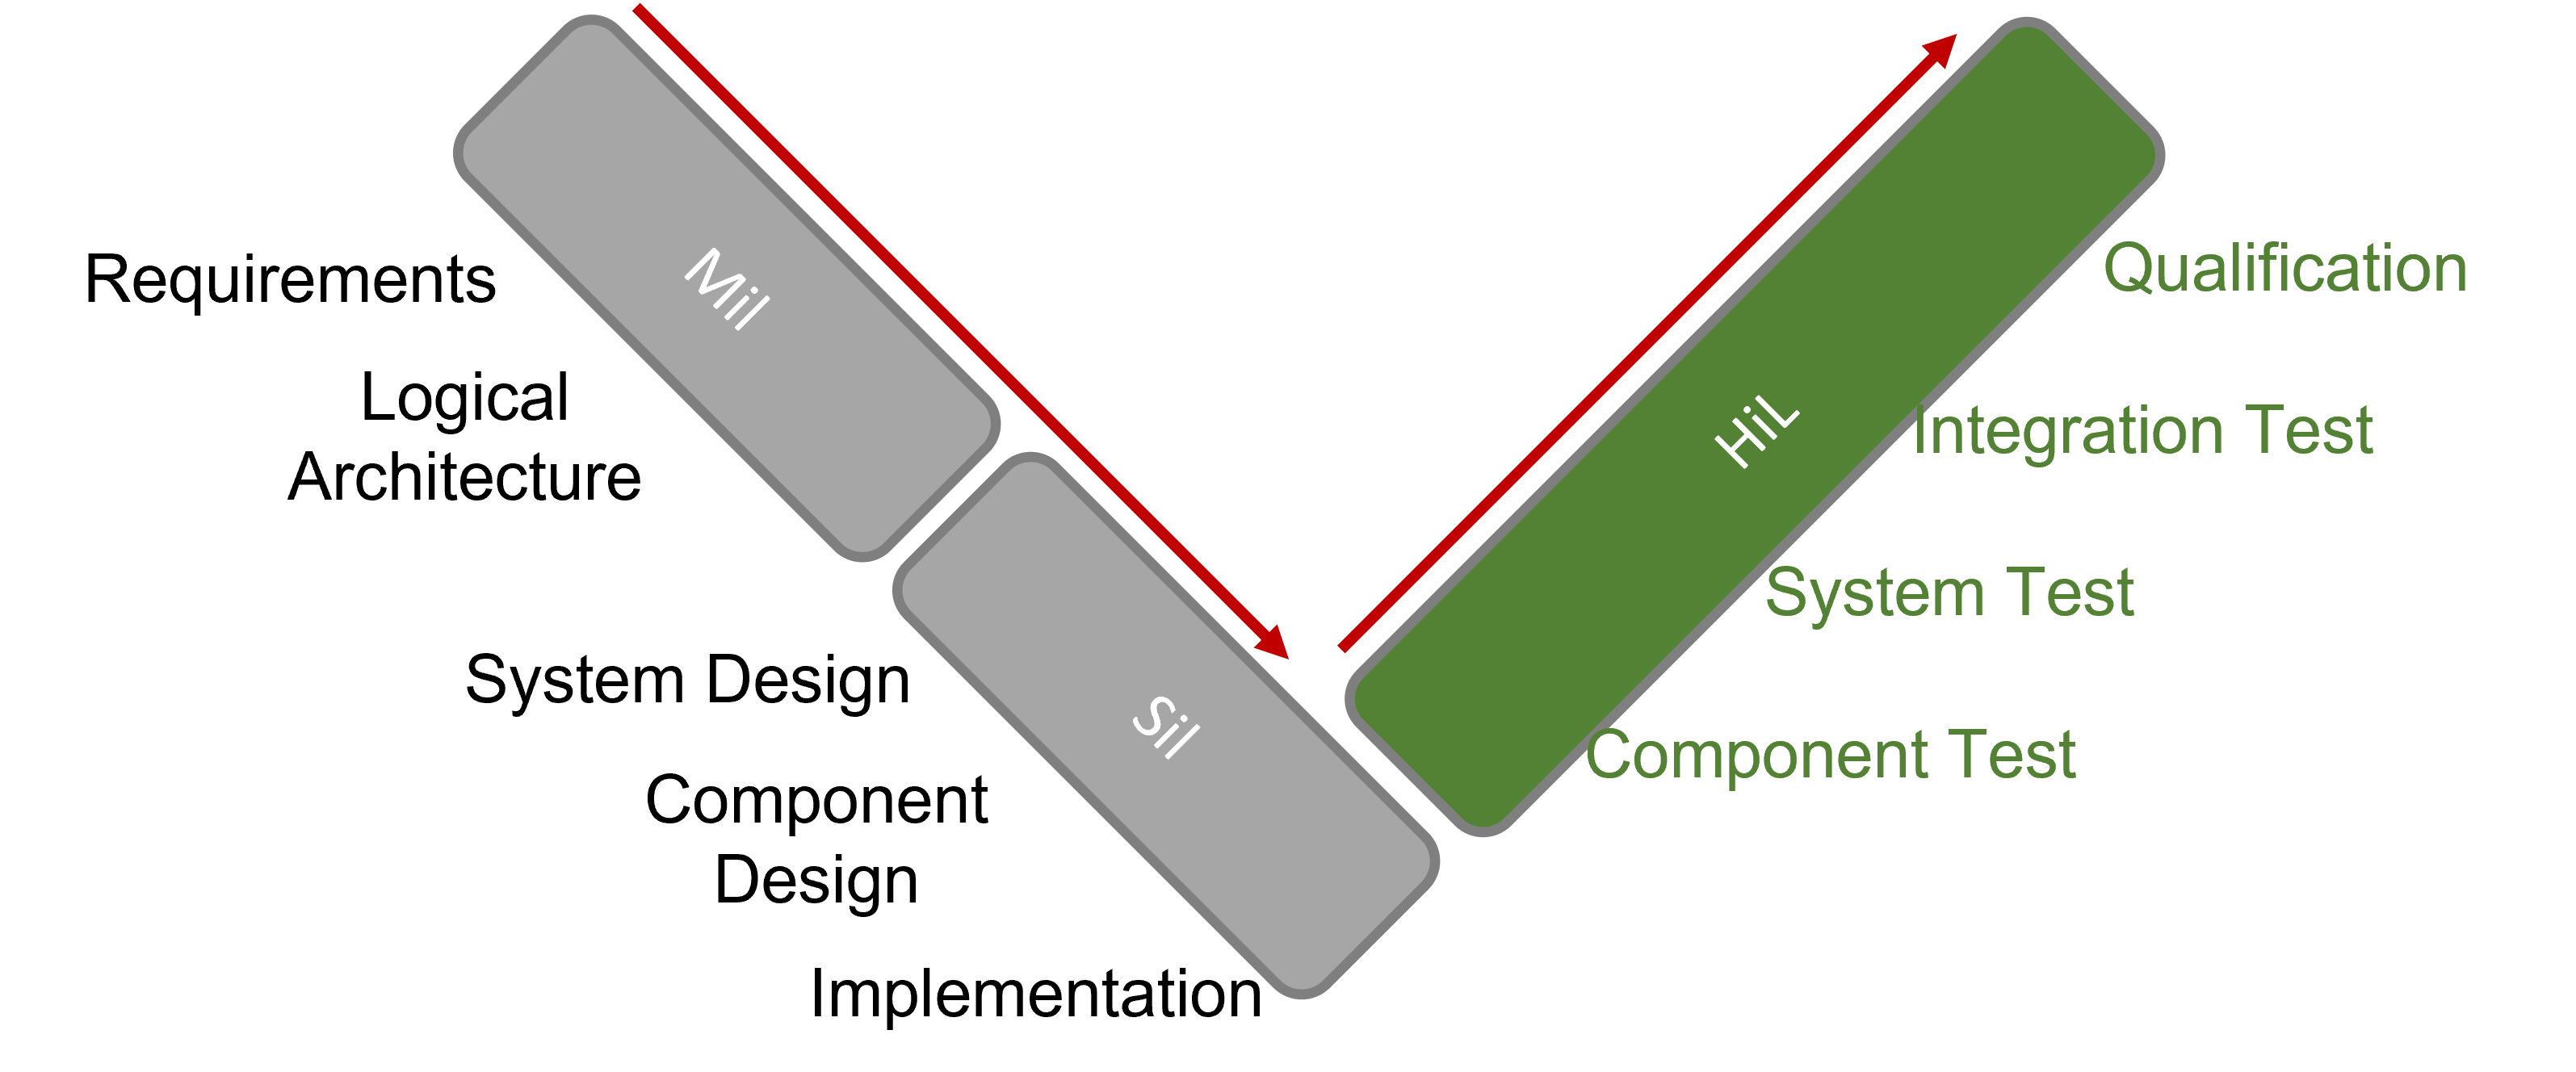
\includegraphics[width=12cm]{Pictures/V Model Component Test.png}
    \caption[V Model Component Test]{V Model Component Test Stage}
    \label{V Model Component Test}
    \end{center}
\end{figure}

\subsection{System Test}
\begin{figure}[h!]
    \begin{center}
    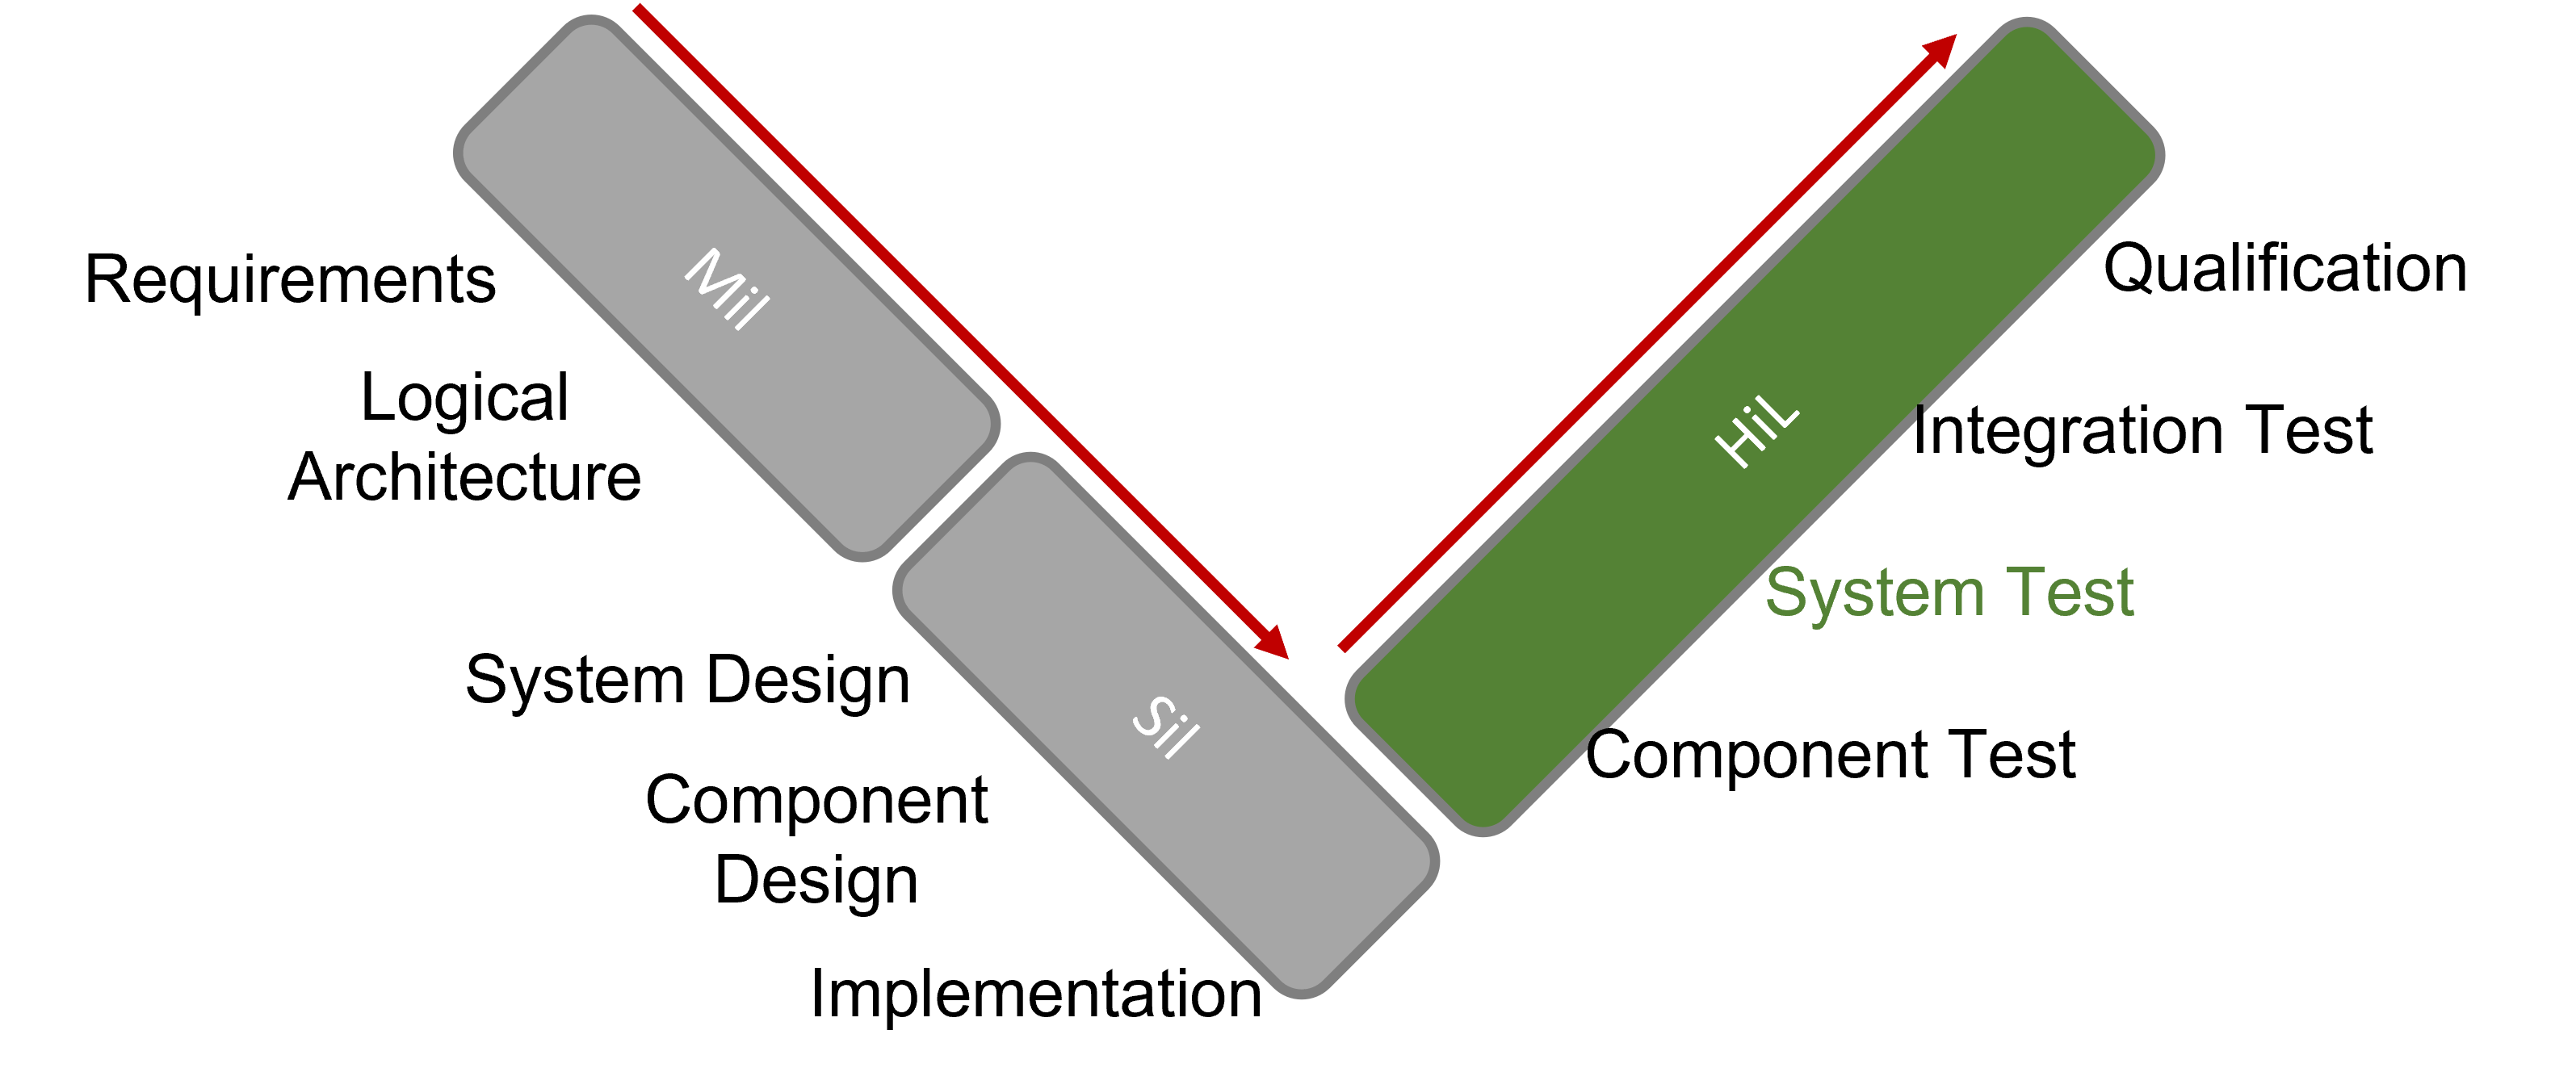
\includegraphics[width=12cm]{Pictures/V Model System Test.png}
    \caption[V Model System Test]{V Model System Test Stage}
    \label{V Model System Test}
    \end{center}
\end{figure}

\subsection{Integration Test}
\subsubsection{Turning}
\subsubsection{Threading}
\begin{figure}[h!]
    \begin{center}
    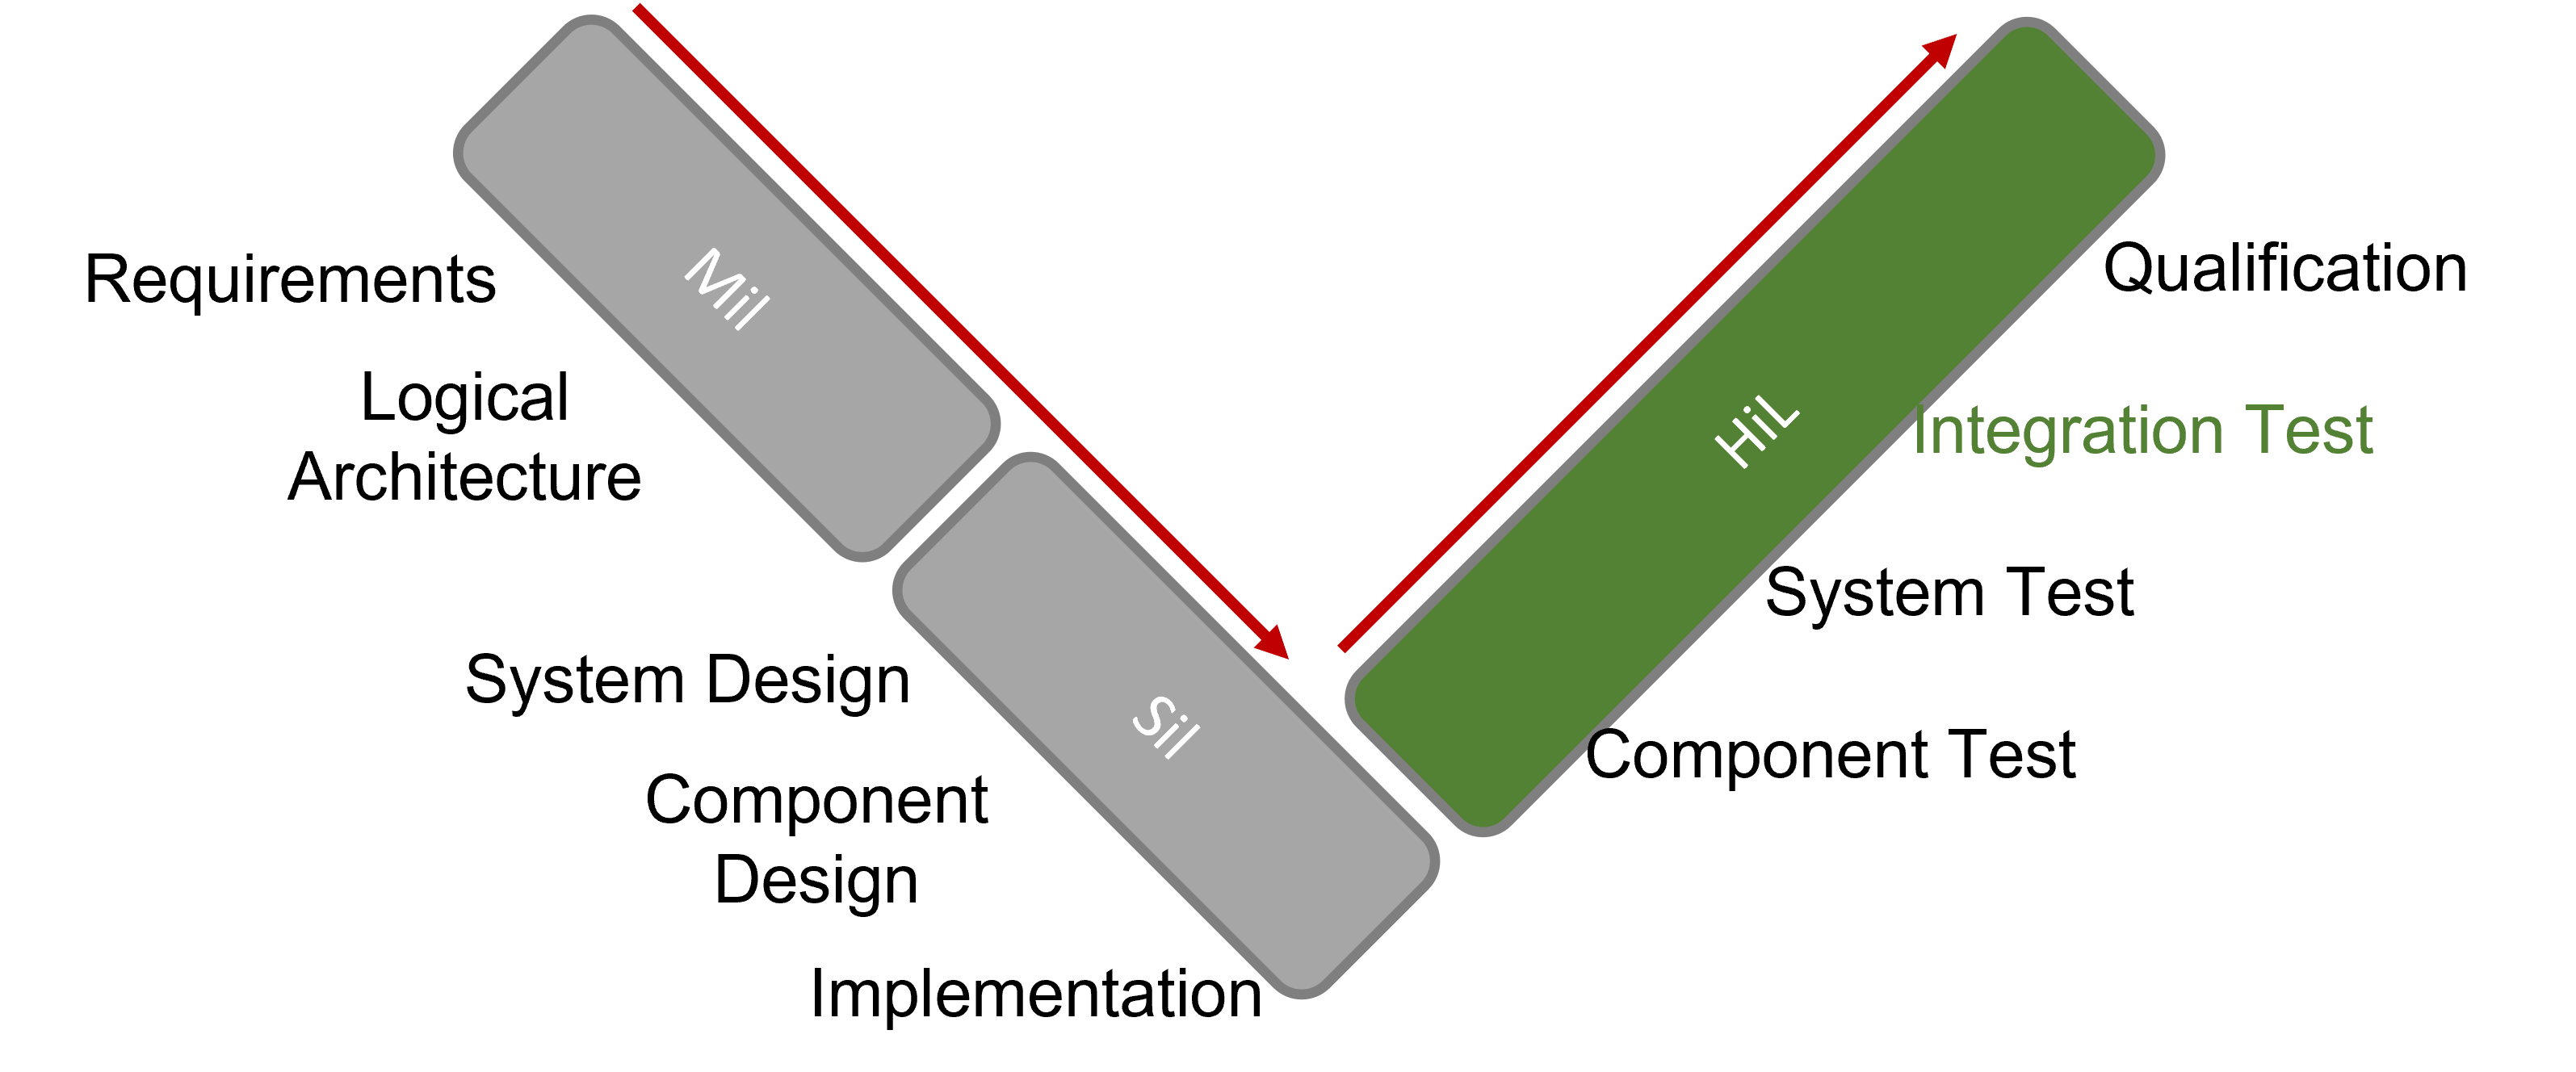
\includegraphics[width=12cm]{Pictures/V Model Integration Test.png}
    \caption[V Model Integration Test]{V Model Integration Test Stage}
    \label{V Model Integration Test}
    \end{center}
\end{figure}













